\documentclass[10pt]{beamer}
\usepackage{amsmath,amssymb}
\usepackage{algorithm,algpseudocode}

\addtobeamertemplate{navigation symbols}{}{%
    \usebeamerfont{footline}%
    \usebeamercolor[fg]{footline}%
    \hspace{1em}%
    \insertframenumber/\inserttotalframenumber
}

\title{Approximating Minimum Subset Feedback Sets in Undirected Graphs with Applications}
\subtitle{Guy Even, Joseph (Seffi) Naor, Baruch Schieber, and Leonid Zosin}

\author{Gustavo Ciotto Pinton}

\institute
{

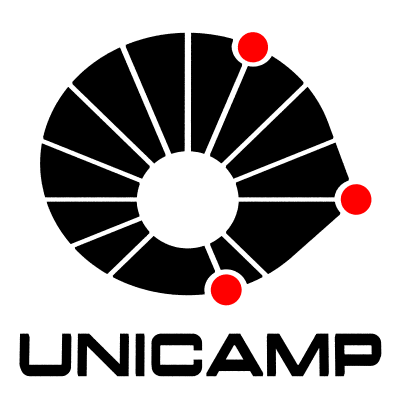
\includegraphics[scale=0.12]{images/logo} \\
\vspace{16pt}
University of Campinas - UNICAMP\\
MO418 - Approximation Algorithms}

\date{November 28th, 2018}

\begin{document}

\begin{frame}
\titlepage
\end{frame}

\begin{frame}
\frametitle{Outline}
\tableofcontents
\end{frame}

\section{Introduction}
\begin{frame}
\frametitle{Introduction}
\framesubtitle{Problem definition}
\begin{itemize}
    \item \(G = (V, E)\) be an undirected graph with a weight function \(w\) associated with either the vertices or edges of \(G\).
    \item A \textbf{feedback vertex set} (FVS) is defined to be a set of vertices that intersects all cycles in \(G\).
    \item A \textbf{feedback edge set} (FES) is defined equally, but in respect to the edges.
    \item SUBSET-FVS or SUBSET-FES: restrict the set of cycles (\textbf{interesting cycles}) that the feedback set should intersect:
    \begin{itemize}
        \item Let \(S \subseteq  V\) be a set of \textit{special} vertices. A cycle is \textbf{interesting} if it contains a \textbf{special} vertex.
    \end{itemize}
    \item We are interested in computing a \textbf{minimum weight subset feedback set}.
\end{itemize}
\end{frame}

\begin{frame}
\frametitle{Introduction}
\framesubtitle{Hardness}
\begin{itemize}
    \item Computing a minimum weight FVS is a classical NP-complete problem [R.M. KARP, \textit{Reducibility among combinatorial problems}].
    \item FES problem can be solved in polynomial time: a minimum weight FES is the complement of a maximum weight
    spanning tree in \(G\) (Kruskal's algorithm).
    \item SUBSET-FES and SUBSET-FVS are NP-complete, even for \(|S| = 1\):
        \begin{itemize}
            \item \textbf{Multiway cut problem}: A multiway cut is a set of edges (or vertices) whose removal disconnects every pair of terminals in \(T \subseteq V\). As seen in class, computing such a minimum cut in \textbf{NP-complete}.
            \item Polynomial time reduction to the subset feedback set problem: connect a single special vertex \(s\) to all \(t \in T\) .
            \item In vertex version, \(s\) has infinite weight. In the edge version, set the weight of all adjacent edges to \(s\) to infinite.
            \item Any cycle passing through \(s\) corresponds to a path connecting two terminals in \(T\).
            \item A subset feedback set with respect to \(s\) is also a multiway cut of \(T\).
        \end{itemize}
\end{itemize}
\end{frame}

\section{Approximating the subset feedback set problem}
\begin{frame}
\frametitle{Approximating the subset SUBSET-FES problem}
\framesubtitle{Some details before the algorithm}
\begin{itemize}
    \item \(G = (V, E)\) be an undirected graph with a weight function \(w : E \rightarrow \mathbb{R}\).
    \item \(S = \{s_1, s_2, \ldots s_k\}\) is the set of special vertices.
    \item Define \(V_i \triangleq V - \{s_i, \ldots, s_k\} \). Consequently, \(V_i \subset V_{i+1}\), \(V_{k+1} = V \) and \(V_1\) is the set of of nonspecial vertices.
    \item Without loss of generality, assume \(G\) is connected and that for each special vertex:
    \begin{itemize}
        \item \(deg(s) = 2\).
        \item Its two neighbors are not special vertices.
        \item its two adjacent edges have infinite weight.
    \end{itemize}
    \item Whenever a vertex \(s\) does not satisfy these conditions:
    \begin{itemize}
        \item For each edge \(e\) adjacent to \(s\), split it in \(e_1\), \(e_2\) and \(e_3\).
        \item Add vertex \(s'\) between \(e_1\) and \(e_2\).
        \item Add vertex \(s''\) between \(e_2\) and \(e_3\).
        \item \(w(e_1) = w(e_2) = \infty\) and \(w(e_3) = w(e)\).
        \item Add \(s'\) to \(S\) and remove \(s\) from this set.
    \end{itemize}
\end{itemize}
\end{frame}

\subsection{Approximating the SUBSET-FES problem}
\begin{frame}
    \frametitle{Approximating the SUBSET-FES problem}
    \framesubtitle{Algorithm}
    \begin{itemize}
        \item Let the two neighbors of \(s_i\) be \(x_i\) and \(y_i\).
        \item Algorithm:
    \end{itemize}
    \begin{algorithm}[H]
        \caption{SUBSET-FES}
        \begin{algorithmic}
            \State $M \leftarrow \emptyset$
            \For {$i = 1$ to $k$}
                \State $M_i \leftarrow \text{minimum cut between \(x_i\) and \(y_i\) in } G_i = (V, E - \cup_{j=1}^{i-1}M_j)$
            \EndFor
            \State $M \leftarrow M_1 \cup M_2 \cup \ldots \cup M_k$
            \State \Return $M$
        \end{algorithmic}
    \end{algorithm}
    \begin{itemize}
        \item The solution is feasible.
    \end{itemize}
\end{frame}

\begin{frame}
    \frametitle{Approximating the SUBSET-FES problem}
    \framesubtitle{Analysis}
    \begin{itemize}
        \item Let OPT denote a minimum weight solution.
        \item Define \(H = (V, E - OPT)\) and \(H_i\) as the subgraph of \(H\) induced by \(V_i\).
        \item \textbf{Fact:} \(H\) does not contain any interesting cycles.
        \item \textbf{Claim:} the number of connected components \(|C|\) in \(H_1\) is \(k + 1\).
        \item \textit{Proof:}
            \begin{itemize}
                \item \(H_1\) consists of connected components: for each special vertex \(s_i\), \(x_i\) and \(y_i\) cannot belong to the same connected component. Otherwise, there would be another interesting cycle.
                \item Build \(H'\) by contracting each component of \(H_1\) into a vertex.
                \item Since \(H\) does not have any cycle, \(H'\) must be a tree.
                \item Number of edges in \(H'\) is \(|E'| = 2k\), since each \(s_i\) has two neighbors.
                \item \textbf{Euler's theorem}: \(|V'| + |F'| = |E'| + 2\). With \(|F'| = 1\) and \(|E'| = 2k \implies |V'| = 2k + 1\).
                \item Therefore \(|C| = |V'| - |S| = k + 1\).
            \end{itemize}
    \end{itemize}
\end{frame}

\begin{frame}
    \frametitle{Approximating the SUBSET-FES problem}
    \framesubtitle{Analysis (II)}
    \begin{itemize}
        \item Connected components of \(H_1\) : \(C_1, \ldots, C_{k+1}\).
        \item Let \(OPT_i\) denote the edges in OPT with one endpoint in \(C_i\).
        \item Each edge in OPT touches two connected components \(\implies \sum_{i=1}^{k+1}w(OPT_i) = 2w(OPT)\).
        \item Injective mapping from {\(M_1, \ldots, M_k\)} to \(C_1, \ldots, C_{k+1}\), i.e., each component can be the image of at most one cut:
        \item For each \(M_i\), we identify \(C_{l(i)}\) and \(C_{r(i)}\):
        \begin{itemize}
            \item \(p\) is  a simple path from \(x_i\) to \(y_i\) in \(G_i = (V, E - \cup_{j=1}^{i-1}M_j)\).
            \item Discard from \(p\) all nonspecial vertices, except for \(x_i\) and \(y_i\). 
            \item The remaining vertices, in order of appearance, are called the \textit{backbone} of \(p\).
            \item Follow the \(backbone\), from \(x_i\) until the first vertex \(v\) that is not connected in \(H_i\) to its subsequent vertex in the backbone.
            \item Such a vertex always exists since the \(p\) is disconnected by OPT.
            \item \(v\) can be either \(x_i\) or a special vertex \(s_j\) such that \(j < i\).
            \item Define \(C_{l(i)} = C_j\) such that \(v \in C_j\).
            \item Define \(C_{r(i)}\) similarly by considering \(p\) in reverse order.
        \end{itemize}
    \end{itemize}
\end{frame}

\begin{frame}
    \frametitle{Approximating the SUBSET-FES problem}
    \framesubtitle{Analysis (III)}
    \begin{itemize}
        \item \textbf{Claim 1:} All simple paths connecting \(x_i\) with \(y_i\) in \(G_i\) have the same backbone.
        \item \textit{Proof}:
        \begin{itemize}
            \item Consider two paths \(p\) and \(q\) and suppose that they have different sequences of special vertices. \item Union of \(p\) and \(q\) must contain an interesting cycle.
            \item Let \(j < i\) be the maximum index of a special vertex in this cycle.
            \item Path connecting \(x_j\) and \(y_j\), obtained by removing \(s_j\) from the cycle, is in \(G_j\).
            \item \(M_j\) must intersect this path and it cannot belong to \(G_i \implies\) contradiction.
        \end{itemize}
    \end{itemize}
\end{frame}

\begin{frame}
    \frametitle{Approximating the SUBSET-FES problem}
    \framesubtitle{Analysis (IV)}
    \begin{itemize}
        \item \textbf{Claim 2:} For \(i = 1, \ldots, k, w(M_i) \leq \min\{w(OPT_{l(i)}), w(OPT_{r(i)})\}\)
        \item \textit{Proof} \(w(M_i) \leq w(OPT_{l(i)})\):
        \begin{itemize}
            \item By Claim 1, all the paths from \(x_i\) to \(y_i\) in \(G_i\) traverse a vertex in \(C_{l(i)}\).
            \item By definition of \(C_{l(i)}\) all these paths emanate from \(C_{l(i)}\) using an edge from \(OPT_{l(i)} \implies\) \(OPT_{l(i)}\) cuts them all.
            \item Since \(M_i\) is a cut of minimum weight, \(w(M_i) \leq w(OPT_{l(i)})\).
        \end{itemize}
        \item \textit{Proof} \(w(M_i) \leq w(OPT_{r(i)})\):
        \begin{itemize}
            \item It can be shown as the previous case.
        \end{itemize}
        \item \textbf{Injective mapping}:
        \begin{itemize}
            \item Auxiliary graph \(H''\): vertex set consists of the the special vertices and one vertex for each connected component of \(H_1\).
            \item \(H''\) is a tree for the same reasons \(H'\) is. It has \(2k\) edges and \(2k + 1\) vertices.
            \item Root this tree at an arbitrary nonspecial vertex.
            \item Each special vertex \(s_i\) has exactly one child which corresponds to either \(C_{l(i)}\) or \(C_{r(i)}\).
            \item Map \(M_i\) to this component.
        \end{itemize}
    \end{itemize}
\end{frame}

\begin{frame}
    \frametitle{Approximating the SUBSET-FES problem}
    \framesubtitle{Results}
    \begin{itemize}
        \item \textbf{Theorem:} Algorithm SUBSET-FES computes a feasible solution whose weight is at most twice the weight of an optimal solution.
        \item \textit{Proof:}
        \begin{itemize}
            \item \(\sum_{i=1}^{k}M_i \leq \sum_{i=1}^{k} \min\{w(OPT_{l(i)}), w(OPT_{r(i)})\}\) (Claim 2)
            \item \(\sum_{i=1}^{k} \min\{w(OPT_{l(i)}), w(OPT_{r(i)})\} \leq \sum_{i=1}^{k} w(OPT_{M(i)})\) (Mapping)
            \item \(\sum_{i=1}^{k} w(OPT_{M(i)}) \leq \sum_{i=1}^{k+1} w(OPT_i) = 2w(OPT)\)  (Definition)
            \item Therefore \(\sum_{i=1}^{k}M_i \leq 2w(OPT)\).
        \end{itemize}
        \item The algorithm is tight.
    \end{itemize}
\end{frame}

\subsection{Approximating the SUBSET-FVS problem}
\begin{frame}
    \frametitle{Approximating the SUBSET-FVS problem}
    \framesubtitle{Analysis}
    \begin{itemize}
        \item With loss of generality, for each special vertex \(s\): \(w(s) = \infty\) and its two neighbors have infinite weight too.
        \item Same approximation algorithm as SUBSET-FES, however:
        \begin{itemize}
            \item \(M_i\) is a minimum weight vertex cut between \(x_i\) and \(y_i\).
            \item Same algorithm as before. In iteration \(i\), \(G_i = (V - \cup_{j=1}^{i-1}M_j, E)\). Return \(\cup_{i=1}^k M_i\).
            \item \(H= (V-OPT, E)\).
            \item \(H_1\) has at least \(k+1\) connected components, denoted by \(C_1, \ldots, C_{k+1}, \ldots, C_n\).
            \item \(OPT_i\) are the vertices in OPT neighbors of \(C_i\).
            \item \(\Delta\) is the maximum vertex degree.
            \item Since every vertex of OPT may be the neighbor of at most \(\Delta\) components, \(\sum_{i=1}^{k+1} w(OPT_i) \leq \Delta w(OPT)\).
            \item By repeating a similar analysis done for SUBSET-FES (finding an injective mapping), we can show that \(\sum_{i=1}^{k} w(M_i) \leq \Delta w(OPT)\).
        \end{itemize}
    \end{itemize}
\end{frame}

\section{Linear Programming Formulation and Integrality Gap}
\begin{frame}
\frametitle{Linear Programming Formulation and Integrality Gap}
\framesubtitle{Definitions}
\begin{itemize}
    \item Given a \textbf{minimization problem}, the integrality gap is defined as 
    \begin{equation*} 
        \text{IG} = \max_{I} \frac{PLI(I)}{PL(I)}
    \end{equation*}
    where \textbf{PLI} is the integer linear problem's solution and \textbf{PL}, its fractional relaxation.
    
    \item \textbf{Integer programming formulation} for FES and FVS:
    \begin{itemize}
        \item Let G = (V,E) be an undirected graph with \(|V| = n\). 
        \item Denote \(\mathcal{C}\) the set of cycles in G.
        \item \(\mathcal{C}_v\) is set of cycles passing through vertex \(v\).
        \item Let \(x_v \in \{0, 1\}\)  (or \(x_e\)) be an indicator variable for membership in a feedback set in G.
    \end{itemize}
\end{itemize}
\end{frame}

\begin{frame}
    \frametitle{Linear Programming Formulation and Integrality Gap}
    \framesubtitle{Formulation for FES and FVS}
    \begin{itemize}
        \item Integer programming formulation for \textbf{FVS}:
        \begin{equation*}
            \begin{array}{ll@{}ll}
                \text{minimize}  & \displaystyle\sum_{v\in V} w(v) * x_v \\
                \text{subject to}& \displaystyle\sum_{v\in C} x_v \geq 1  \text{ for every } C \in \mathcal{C}\\
                                    & x_v \in \{0, 1\} \text{ for every } v \in V\\
            \end{array}
        \end{equation*}

        \item Integer programming formulation for \textbf{FES}:
        \begin{equation*}
            \begin{array}{ll@{}ll}
                \text{minimize}  & \displaystyle\sum_{e\in E} w(e) * x_e \\
                \text{subject to}& \displaystyle\sum_{e\in C} x_e \geq 1  \text{ for every } C \in \mathcal{C}\\
                                    & x_e \in \{0, 1\} \text{ for every } e \in E\\
            \end{array}
        \end{equation*}
\end{itemize}
\end{frame}
    
\begin{frame}
    \frametitle{Linear Programming Formulation and Integrality Gap}
    \framesubtitle{Formulation for SUBSET-FES and SUBSET-FVS}
    \begin{itemize}
        \item We can extend the previous problems to consider only the cycles containing the special vertices \(S\).
        \item Integer programming formulation for \textbf{SUBSET-FVS}:
        \begin{equation*}
            \begin{array}{ll@{}ll}
                \text{minimize}  & \displaystyle\sum_{v\in V} w(v) * x_v \\
                \text{subject to}& \displaystyle\sum_{v\in C} x_v \geq 1  \text{ for every } C \in \bigcup_{s\in S} \mathcal{C}_s\\
                                 & x_v \in \{0, 1\} \text{ for every } v \in V\\
            \end{array}
        \end{equation*}

        \item Integer programming formulation for \textbf{SUBSET-FES}:
        \begin{equation*}
            \begin{array}{ll@{}ll}
                \text{minimize}  & \displaystyle\sum_{e\in E} w(e) * x_e \\
                \text{subject to}& \displaystyle\sum_{e\in C} x_e \geq 1  \text{ for every } C \in \bigcup_{s\in S} \mathcal{C}_s\\
                                    & x_e \in \{0, 1\} \text{ for every } e \in E\\
            \end{array}
        \end{equation*}
\end{itemize}
\end{frame}

\begin{frame}
    \frametitle{Linear Programming Formulation and Integrality Gap}
    \framesubtitle{Integrality Gap for FES and FVS}

    \begin{itemize}
        \item Let's show that the integrality gap in the FVS and FES can be as big as \(\Omega(\log|V|)\). 
        \begin{itemize}
            \item Let \(H_n = (V,E)\) be a connected, 3-regular graph, with \(|V(H_n)| = n\) and girth of \(H_n\) is \(\lceil \log n \rceil\).
            \item Such graphs exist and can be constructed explicitly. (See, e.g., Bollobás [6, pp. 108–110]).
            \item Set all weights (edges or vertices) in G to 1.
            \item \textbf{Claim 1:} \textit{The value of the optimal fractional FVS solution in \(H_n\) is at most \(\frac{n}{\lceil \log n \rceil }\). The value of the optimal fractional FES solution in \(H_n\) is at most \(1.5\frac{n}{\lceil \log n \rceil}\).}
            \item \textit{Proof:} 
                \begin{itemize} 
                    \item Length of the shortest cycle contained in G is \(\lceil \log n \rceil\).
                    \item A feasible fractional solution for FVS could be \(x_v = \frac{1}{\lceil \log n \rceil} \forall v \in V\). Its cost is \(\displaystyle\sum_{v\in V} w(v) * x_v  = \displaystyle\sum_{v\in V} \frac{1}{\lceil \log n \rceil} = \frac{n}{\lceil \log n \rceil}\)
                    \item For FES, it could be \(x_e = \frac{1}{\lceil \log n \rceil} \forall e \in E\). 
                    \item \(|E| = 1.5n\), since \(\displaystyle\sum_{v\in V} deg(v) = 2|E|\) and \(deg(v) = 3\) \(\forall v \in V\).
                    \item Therefore, FES solution's cost would be
                    \(\displaystyle\sum_{e\in E} w(e) * x_e = 1.5\frac{n}{\lceil \log n \rceil}\).
                \end{itemize}
        \end{itemize}
    \end{itemize}
\end{frame}

\begin{frame}
    \frametitle{Linear Programming Formulation and Integrality Gap}
    \framesubtitle{Integrality Gap for FES and FVS (II)}
    \begin{itemize}
        \item An optimal integral solution for the FES is the complement of any spanning tree of \(H_n\).
        \item Its cost is \(1.5n - (n - 1) = \frac{n}{2} + 1\).
        \item Therefore, \(IG_{FES} = \frac{\frac{n}{2} + 1}{1.5\frac{n}{\lceil \log n \rceil}} = \lceil \log n \rceil \frac{n+2}{3n}\), which is \(\Omega(\log |V|)\).
        \item \textbf{Claim 2:} \textit{The value of an optimal integral solution for the FVS problem in \(H_n\) is \(\Omega(n)\).}
        \item \textit{Proof:} 
        \begin{itemize}
            \item An optimal solution to the FES problem costs at most \(\Delta = 3\) times the cost of an optimal solution to the FVS problem.
            \item Therefore, the cost of the FVS is at least \(\frac{\frac{n}{2} + 1}{3} = \frac{n}{6} + \frac{1}{3}\), which is \(\Omega(n)\).
        \end{itemize}
        \item We have then \(IG_{FVS} = \frac{\frac{n}{6} + \frac{1}{3}}{\frac{n}{\lceil \log n \rceil}} = \lceil \log n \rceil \frac{n+2}{6n}\), which is also \(\Omega(\log |V|)\).
    \end{itemize}
\end{frame}

\begin{frame}
    \frametitle{Linear Programming Formulation and Integrality Gap}
    \framesubtitle{Integrality Gap for SUBSET-FES and SUBSET-FVS}
    \begin{itemize}
        \item Let \(F_n\) be the union of two graphs:
        \begin{itemize}
            \item \(H_k = (S,E)\), with \(|S| = k\).
            \item Clique \(C_{n-k}\) on the remaining \(n-k\) vertices.
        \end{itemize}
        \item Connect \(H_k\) and \(C_{n-k}\) by a \textit{single} edge.
        \item No cycle that goes through a vertex in \(S\) intersects the clique.
        \item Thus, for integrality gap, consider only \(H_k\) which has \(k\) vertices.
        \item By using claims 1 and 2, we obtain that \(IG_{SUBSET-FES}\) and \(IG_{SUBSET-FVS}\) are in \(\Omega(\log k)\).
    \end{itemize}
\end{frame}

\end{document}